\chapter{Psalm 20}

\begin{figure}
  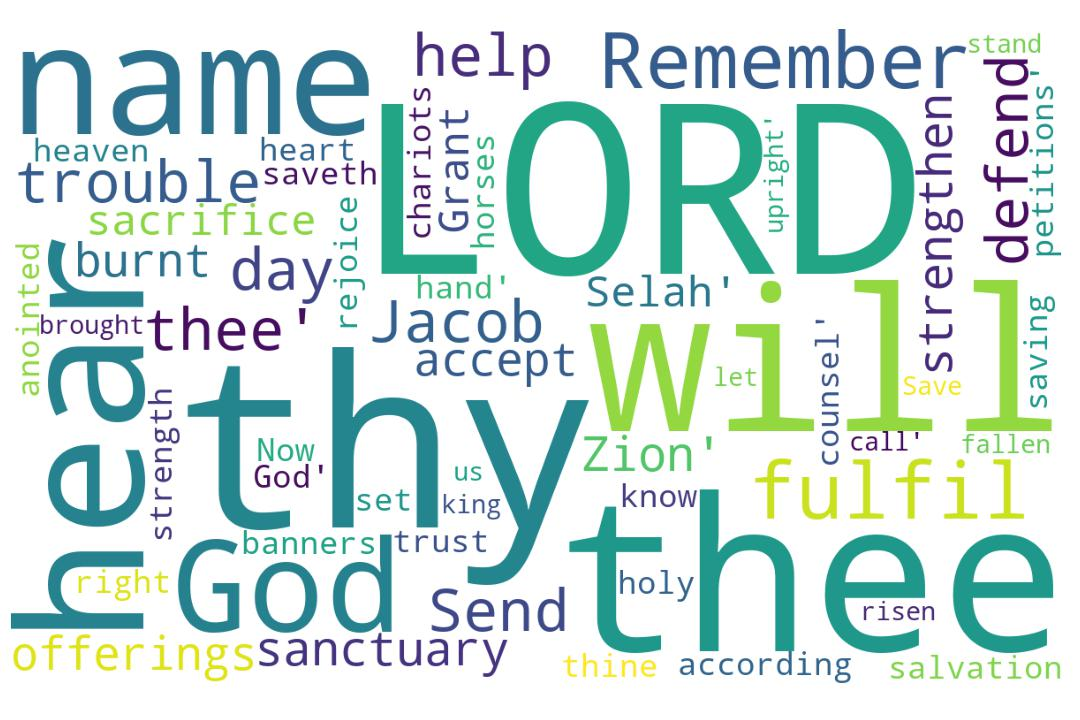
\includegraphics[width=\linewidth]{19OT-Psalms/Psalm20-WordCloud.jpg}
  \caption{Psalm 20 Word Cloud}
  \label{fig:Psalm 20 word Cloud}
\end{figure}

\marginpar{\scriptsize \centering \fcolorbox{bone}{lime}{\textbf{MY SAVIOUR}}\\ (Psalm 20:1-9) \begin{compactenum}[I.][8]
    \item Is a Savior that \textbf{Hears} \index[scripture]{Psalms!Psa 020:01}\index[scripture]{Psalms!Psa 020:09}(Psa 20:1,9)
    \item Is a Savior that \textbf{Helps} \index[scripture]{Psalms!Psa 020:02}(Psa 20:2)
    \item Is a Savior that \textbf{Honors} \index[scripture]{Psalms!Psa 020:03}(Psa 20:3)
    \item Is a Savior that has a \textbf{Heart} for his People \index[scripture]{Psalms!Psa 020:04}\index[scripture]{Psalms!Psa 020:04}(Psa 20:4)
    \item Is a Savior that provids \textbf{Hope} \index[scripture]{Psalms!Psa 020:05}(Psa 20:5)
    \item Is a Savior that has a \textbf{Heritage}  \index[scripture]{Psalms!Psa 020:06}(Psa 20:6)
    \item Is a Savior that is on \textbf{High}  \index[scripture]{Psalms!Psa 020:06}(Psa 20:6)
\end{compactenum}}

\footnote{\textcolor[cmyk]{0.99998,1,0,0}{\hyperlink{TOC}{Return to end of Table of Contents.}}}\footnote{\href{https://www.audioverse.org/english/audiobibles/books/ENGKJV/O/Ps/1}{\textcolor[cmyk]{0.99998,1,0,0}{Psalms Audio}}}\textcolor[cmyk]{0.99998,1,0,0}{To the chief Musician, A Psalm of David.}\\
\\
\textcolor[cmyk]{0.99998,1,0,0}{The LORD \fcolorbox{bone}{lime}{hear} thee in the day of trouble; the name of the God of Jacob defend thee;}\footnote{\textbf{Daniel 12:1} -- And at that time shall Michael stand up, the great prince which standeth for the children of thy people: and there shall be a time of trouble, such as never was since there was a nation \emph{even} to that same time: and at that time thy people shall be delivered, every one that shall be found written in the book.}\footnote{\textbf{Matthew 24:21} -- For then shall be great tribulation, such as was not since the beginning of the world to this time, no, nor ever shall be.}
[2] \textcolor[cmyk]{0.99998,1,0,0}{Send thee \fcolorbox{bone}{lime}{help} from the sanctuary, and strengthen thee out of Zion;}
[3] \textcolor[cmyk]{0.99998,1,0,0}{Remember all \fcolorbox{bone}{lime}{thy offerings}, and accept thy burnt sacrifice; Selah.}
[4] \textcolor[cmyk]{0.99998,1,0,0}{Grant thee according to thine own \fcolorbox{bone}{lime}{heart}, and fulfil all thy counsel.}
[5] \textcolor[cmyk]{0.99998,1,0,0}{We will rejoice in thy salvation, and in the name of our God we will set up \emph{our} banners: the LORD \fcolorbox{bone}{lime}{fulfil} all thy petitions.}
[6] \textcolor[cmyk]{0.99998,1,0,0}{Now know I that the LORD saveth his anointed; he will hear him from his holy heaven with the saving strength of his right hand.}\footnote{\textbf{Psalm 17:7} -- Shew thy marvellous lovingkindness, O thou that savest by thy right hand them which put their trust \emph{in thee} from those that rise up \emph{against them.}}\footnote{\textbf{Psalm 139:10} -- Even there shall thy hand lead me, and thy right hand shall hold me.}
[7] \textcolor[cmyk]{0.99998,1,0,0}{Some \emph{trust} in chariots, and some in horses: but we will remember the name of the LORD our God.}\footnote{Kidner points out that while chariots and horses were the most formidable force of ancient times, here the verse induces memories of Israel's vicotries at the Red Sea (Exodus 14) and at the river Kishon (Judges 4). but we will remember the name of the LORD our God. \cite{kidner2014psalmsV1} }\footnote{\textbf{Exodus 14:28-29} -- And the waters returned, and covered the chariots, and the horsemen, and all the host of Pharaoh that came into the sea after them; there remained not so much as one of them. [29] But the children of Israel walked upon dry land in the midst of the sea; and the waters were a wall unto them on their right hand, and on their left.}\footnote{\textbf{Judges 4:15-15} -- And the LORD discomfited Sisera, and all his chariots, and all his host, with the edge of the sword before Barak; so that Sisera lighted down off his chariot, and fled away on his feet. [16] But Barak pursued after the chariots, and after the host, unto Harosheth of the Gentiles: and all the host of Sisera fell upon the edge of the sword; and there was not a man left.} 
[8] \textcolor[cmyk]{0.99998,1,0,0}{They are brought down and fallen: but we are risen, and stand upright.}
[9] \textcolor[cmyk]{0.99998,1,0,0}{Save, LORD: let the king \fcolorbox{bone}{lime}{hear} us when we call.}
